\section{Introduction}
\label{sec:introduction}

Two research groups evaluate the same model, prompt, and financial benchmark. One reports 11\% accuracy; the other reports 44\%. The difference is not the model output, but the regular expression used to extract its answer. This is not hypothetical: across seven major evaluation frameworks, we find no shared, documented extraction protocol, and several frameworks do not fully specify their procedure. A benchmark score without its extraction methodology is therefore not reproducible.

Most evaluation harnesses extract a numeric answer from free-form model output using regular expressions. For example, \numparser{} selects the first number following an equals sign. If the model instead places its answer in \boxedparser{} or elsewhere in its reasoning trace, extraction may fail silently, recording a correct response as incorrect. Intentionally incompatible parsers can therefore produce extreme differences; we treat this as a sanity check rather than our main result.

Our focus is the less obvious sensitivity that remains among broadly format-compatible parsers. We distinguish the full parser spread (Res-A) from a stricter residual spread that excludes both \numparser{} and the format-specific \boxedparser{} (Res-B). Across four mathematical benchmarks, Res-B ranges from 1--7\pp{}. Across two financial benchmarks, it ranges from 3--19\pp{}, with the largest effect on FinQA using Qwen3-8B. A manual audit links this sensitivity to financial surface forms, answer normalization, and the placement of intermediate and final values in multi-step reasoning. Parser choice can also change model rankings: on FinQA, some parser pairs fully reverse the ordering of the evaluated models.

This sensitivity matters because extraction practices vary substantially across the evaluation ecosystem. FinQA uses program execution and string comparison documented in released code~\cite{chen2021finqa}; FinanceReasoning uses GPT-4o-mini as an LLM judge~\cite{zhang2025financereasoning}; PIXIU parses text following an ``Answer:'' marker~\cite{xie2023pixiu}; FinBen delegates evaluation to lm-eval-harness without specifying its extraction procedure in the paper~\cite{xie2024finben}; and OpenCompass~\cite{opencompass2023} does not fully document its extraction method. Tolerance thresholds and normalization rules also differ. Consequently, nominally comparable benchmark scores may reflect different measurement procedures.

We make four contributions:
\begin{enumerate}
    \item \textbf{Ecosystem audit.} We document answer-extraction practices across seven major evaluation frameworks and identify substantial gaps in protocol standardization and reporting (Section~\ref{sec:parser_audit}).

    \item \textbf{Cross-domain sensitivity analysis.} Using five parsers, three models, and six benchmarks, we show that residual parser sensitivity reaches 3--19\pp{} on the evaluated financial benchmarks, compared with 1--7\pp{} on mathematical controls (Section~\ref{sec:results}).

    \item \textbf{Ranking and failure analysis.} We show that no parser is uniformly optimal, that parser choice can reverse model rankings, and that the observed disagreements arise from several distinct formatting and normalization failures (Sections~\ref{sec:finance_challenges} and~\ref{sec:results}).

    \item \textbf{Evaluation protocol.} We propose canonical answer formats, extraction-method disclosure, parser code release, multi-parser sensitivity reporting, and targeted auditing of parser disagreements (Section~\ref{sec:impl_benchmark}).
\end{enumerate}

We evaluate Qwen3-1.7B and Qwen3-8B on all six benchmarks, and GLM-4-9B-Chat on the financial benchmarks for cross-family validation. Together, the results establish answer extraction as a consequential measurement variable rather than a minor implementation detail. The remainder of this paper is organized as follows. Section~\ref{sec:background} surveys related work on financial LLM benchmarks and evaluation methodology. Section~\ref{sec:parser_audit} presents the benchmark ecosystem audit. Section~\ref{sec:finance_challenges} presents the finance-specific failure taxonomy. Section~\ref{sec:setup} describes our experimental design. Section~\ref{sec:results} reports the cross-domain comparison. Section~\ref{sec:implications} discusses implications and presents the recommended extraction protocol. Section~\ref{sec:conclusion} concludes.

\begin{figure*}[htb!]
\centering
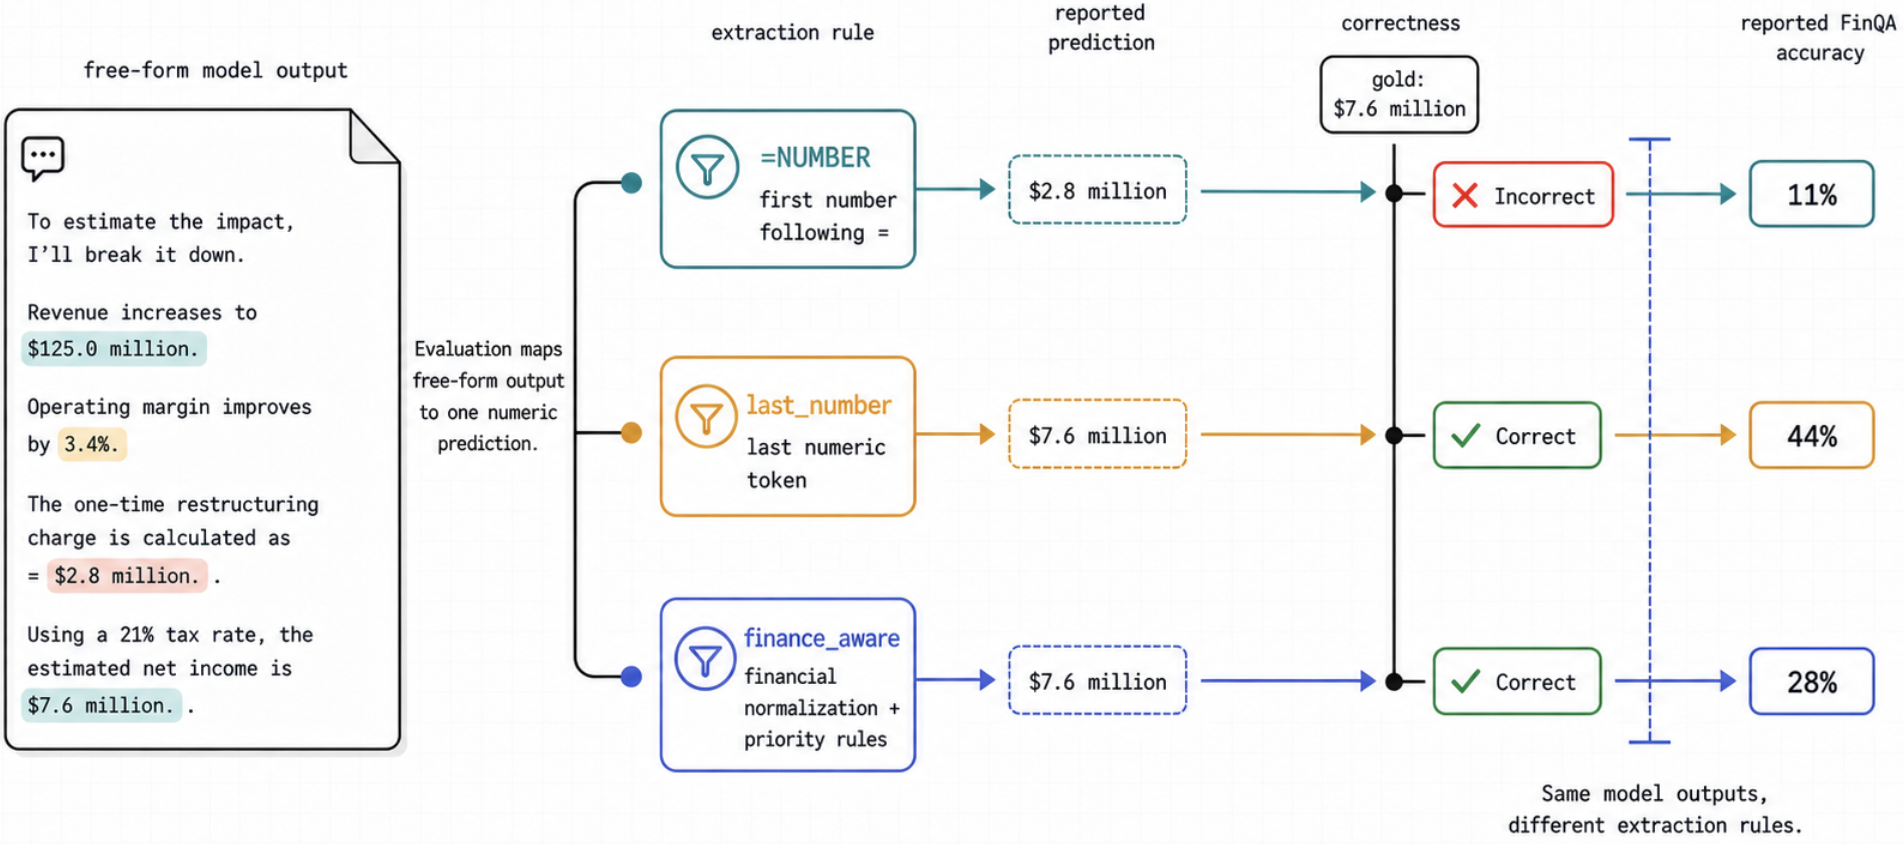
\includegraphics[width=0.85\textwidth]{figures/teaser.png}
\caption{Answer extraction as a hidden measurement variable. Different extraction rules applied to identical model outputs can produce substantially different reported accuracies.}
\label{fig:teaser}
\end{figure*}
